\documentclass[12pt, a4paper]{article}
%\usepackage[german,ngerman]{babel} 
\usepackage[utf8]{inputenc}
\usepackage[T1]{fontenc}
\usepackage{lmodern}
\usepackage{amsmath}
\usepackage{geometry}
\usepackage{subfigure}
\usepackage{graphicx}
\geometry{
  left=2.7cm,
  right=2.7cm,
  top=3cm,
  bottom=3cm,
  bindingoffset=5mm
}
\graphicspath {{images/}}

\begin{document}
% ========== TITLEPAGE ==========
\pagenumbering{gobble}

\begin{titlepage} 						%Start of title page.
\centering								%Horizontally centre the page. 

\begin{center}
	
\includegraphics[width=0.5\textwidth]{universitaet-innsbruck-logo-cmyk-farbe} \\
	Leopold-Franzens-Universität Innsbruck
\end{center}

\vfill

\Huge{Assignment 1 - Report}

\vspace{0.5cm}

\Large{Computer Haptics}

\vfill
\hfill

\begin{center}
\textbf{Group 6} \\
Thibault Gerrier \\
Philipp Häusle \\
Daniel Linter \\
\vspace{0.5cm}
\textbf{Other Group} \\
Thomas Tschol \\

\vspace*{\fill}

\end{center}

\begin{center}
	\today
\end{center}

\end{titlepage}	
\pagenumbering{arabic}
% ========== ALL OTHER SITES ==========
\section{Assembly} \label{sec:ass}
During assembly we ran into a few difficulties: Which screws, nuts and washers to use was often unclear, we had to try different thicknesses, lengths and combinations of nuts. Another problem was fixing the motor to the "main upward plastic thing", using the appropriate screws didn't work, as they didn’t hold on to the plastic. We needed to use some washers, so that the screws wouldn’t "fall through". Other than that the assembly was fine and we were able to assembly the hapkit device.

\begin{table}[t]
\centering
\begin{tabular}{|r|r|}
\hline
Degrees & Readings \\ \hline
-50 & -3,590 \\ \hline
-40 & -3,070 \\ \hline
-30 & -2,290 \\ \hline
-20 & -140 \\ \hline
-10 & -560 \\ \hline
0 & 259 \\ \hline
10 & 1,150 \\ \hline
20 & 2,050 \\ \hline
30 & 2,940 \\ \hline
40 & 3,840 \\ \hline
50 & 4,350 \\ \hline
\end{tabular}
\caption{Measured values for degrees}
\label{table:readings}
\end{table}

\section{Calibration} \label{sec:cal}
Our readings after running the given example code on the haptic device can be seen in Table~\ref{table:readings}. We also plotted these readings in Figure~\ref{fig:readings_plot}. As expected a linear function emerged from our readings. To note is that the values for 50 and -50 degrees are slightly off curve, since the readings occurred a little before \& after 50 degrees, since the haptik device doesn’t quite reach the 50 mark.

We took our results and calculated values for a and b of the regression equation
\begin{equation*}
X_m = a * update_{pos} + b
\end{equation*}

We found the values: $a = -3.97074$ and $b = 0.01197$. Using these values we can calculate degrees based on the readings of the haptic device.

\begin{equation*}
degrees = a * reading + b
\end{equation*}

With those degrees we can further calculate the distance in radians of the position $X_m$ in milimetres.

\begin{equation*}
distance = angle / 360 * 2 * PI * radius
\end{equation*}


\begin{figure}
	\centering
	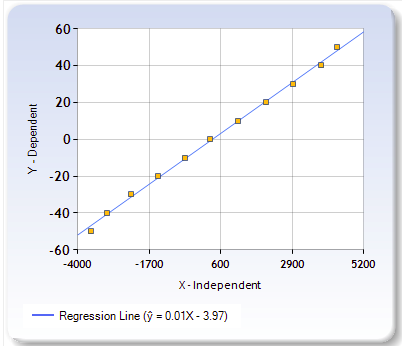
\includegraphics[width=0.5\textwidth]{readings_plot}
	\caption{The plot depicting the received linear function.}
	\label{fig:readings_plot}
\end{figure}


% ========== BIBLIOGRAPHY ==========
%\bibliographystyle{plain}
%\bibliography{literature}
\end{document}
